

La plataforma de Android nos ofrece mecanismos para conservar la vida de la batería. De forma que nos ofrece diversas APIs para planificar los procesos, describimos algunas en la sección de APIs \cite{jobdispatcher}.

Dejando las APIs a un lado, caben destacar  dos funciones de ahorro de energía que presenta Android, ya que estas prolongan la vida de la batería administrando la forma en que las apps se comportan cuando un dispositivo no está conectado a una fuente de energía. Descanso reduce el consumo de batería aplazando la actividad de CPU y de red de las apps en segundo plano cuando el dispositivo no se usa durante períodos de tiempo prolongados. App Standby aplaza la actividad de red en segundo plano de las apps con las cuales el usuario no haya interactuado recientemente.

A continuación vamos a profundizar en ambas funciones.

\paragraph{Modo Descanso:}

Si un usuario deja un dispositivo desconectado, quieto y con la pantalla apagada durante un período de tiempo determinado, este entra en el modo Descanso. En el modo Descanso, el sistema intenta conservar la carga de la batería restringiendo el acceso por parte de las apps a servicios de uso intenso de red y CPU. También evita que las apps accedan a la red y aplaza sus tareas, sincronizaciones y alarmas estándares.

De forma periódica, el sistema desactiva el modo Descanso durante un tiempo breve para permitir que las apps completen sus actividades aplazadas. Durante este período de mantenimiento, el sistema ejecuta todas las sincronizaciones, tareas y alarmas pendientes, y permite que las apps accedan a la red.
\begin{figure}[h]
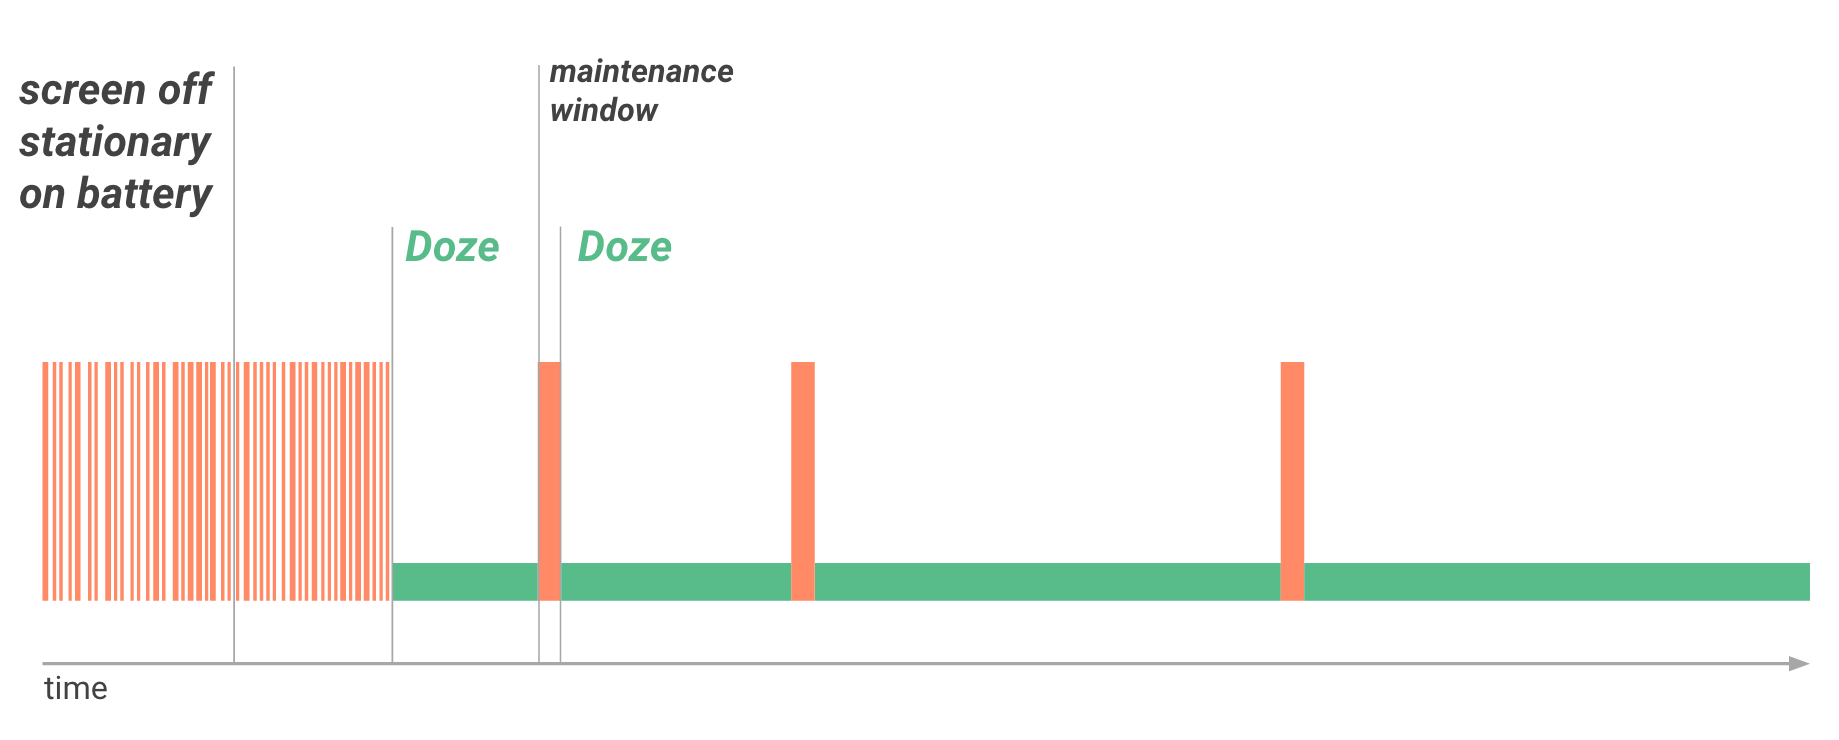
\includegraphics[scale=0.20]{imagenes/doze.png} 
\floatfoot{Figura 5: Descanso proporciona un período de mantenimiento recurrente para que las apps usen la red y controlen actividades pendientes.}
\end{figure}



Al finalizar cada período de mantenimiento, el sistema vuelve a activar el modo Descanso, suspender el acceso a la red y aplazar tareas, sincronizaciones y alarmas. Con el paso del tiempo, el sistema programa los períodos de mantenimiento cada vez con menos frecuencia, lo cual permite reducir el consumo de batería en casos de inactividad durante más tiempo cuando el dispositivo no está conectado a un cargador.

Si bien el usuario activa el dispositivo moviéndolo, encendiendo la pantalla o conectándolo a un cargador, el sistema desactiva el modo Descanso y todas las apps vuelven a la actividad normal.

\paragraph{Restricciones del modo Descanso:}
Durante el modo Descanso, se aplican las siguientes restricciones a tus apps:
\begin{enumerate}
\item Se suspende el acceso a la red.
\item El sistema ignora los wake locks.
\item Las alarmas estándares AlarmManager (incluidas setExact() y setWindow()) se aplazan hasta el siguiente período de mantenimiento.
\begin{enumerate}
\item Si necesitas programar alarmas que se activen en el modo Descanso, usa setAndAllowWhileIdle() o setExactAndAllowWhileIdle().
\item Las alarmas programadas con setAlarmClock() se activan con normalidad; el sistema desactiva el modo Descanso antes de que esas alarmas se activen.
\end{enumerate}
\item El sistema no realiza escaneos de Wi-Fi.
\item El sistema no permite que se ejecuten adaptadores de sincronización.
\item El sistema no permite que se ejecute JobScheduler.
\end{enumerate}

\paragraph{Información sobre App Standby}

El modo App Standby permite que el sistema determine si una app se encuentra inactiva cuando el usuario no la usa activamente. El sistema hace esta determinación cuando el usuario no aplica toques en la app durante un período determinado y cuando no rige ninguna de las siguientes condiciones:
\begin{enumerate}

\item El usuario inicia explícitamente la app.
\item La app actualmente tiene un proceso en primer plano (ya sea como actividad o como servicio en primer plano, o en uso por parte de otra actividad u otro servicio en primer plano).
\item La app genera una notificación que los usuarios ven en la pantalla bloqueada o en la bandeja de notificaciones.
\end{enumerate}

Cuando el usuario enchufa el dispositivo en una fuente de energía, el sistema libera las apps del estado de reposo, con lo cual les permite acceder libremente a la red y ejecutar cualquier tarea y sincronización pendientes. Si el dispositivo queda inactivo durante períodos prolongados, las apps inactivas pueden acceder a la red aproximadamente una vez al día.

\paragraph{Firebase Cloud Messaging}

Para poder utilizar nuestra aplicación en ambos modos de ahorro de batería utilizaremos la solución de mensajería  Firebase Cloud Messaging \cite{FIREBASECLOUDMESS}, la cual nos permitirá enviar mensajes de forma segura al backend aún estando en ahorro de energía. Nos resultará sencilla su implementación al ya tener Firebase integrado en nuestra aplicación.
